\chapter{Datensatz}
\label{chap:Datensatz}
\pagestyle{plain}

Untersuchungsgrundlage der Hausarbeit sind die zwei im Folgenden vorgestellten Chor-Arrangements. Die Noten der beiden Stücke befinden sich in ihrer Gesamtheit im \nameref{chap:Anhang}. An dieser Stelle werden nur Text und für die Ausarbeitung relevante Ausschnitte der Noten präsentiert.

\section{Run To You}

Bei dem ersten Stück handelt es sich um \textit{Run To You}, geschrieben von der A Cappella Gruppe \textit{Pentatonix} in Zusammenarbeit mit Ben Bram. \textit{Run To You} ist ein fünfstimmiges Chor-Arrangement für Sopran, Alt, Tenor, Bariton und Bass. Das Stück ist aufgeteilt in zwei Strophen (Studierziffern A und C), gefolgt von jeweils einem Refrain (Studierziffern B und D). Der zweite Refrain mündet in die Bridge (Studierziffer E). Das Stück endet mit einem leicht veränderten Refrain (Studierziffer F), dessen Ende gesummt wird.

\subsection*{Text}

\begin{verbatim}
[Strophe 1]
A light in the room
It was you who was standing there
Tried, it was true
As your glance met my stare
But your heart drifted off
Like the land split by sea
I tried to go, to follow
To kneel down at your feet

[Refrain]
I'll run, I'll run, I'll run, run to you
I'll run, I'll run, I'll run, run to you

[Strophe 2]
I've been settling scores
I've been fighting so long
But I've lost your war
And our kingdom is gone
How shall I win back your heart
Which was mine?
I have broken bones
And tattered clothes
I've run out of time

[Refrain]

[Bridge]
Oh, I will break down the gates of heaven
A thousand angels stand waiting for me
Oh take my heart and I'll lay down my weapons
Break my shackles to set me free

[Refrain]
\end{verbatim}

\subsection*{Melodie}

In diesem Stück alterniert die Melodie-Stimme zwischen Tenor und Alt. Die Strophen (Studierziffern A und C) werden von der Tenor-Stimme, Refrain und Bridge (Studierziffern B, D, E, F) von der Alt-Stimme geführt.

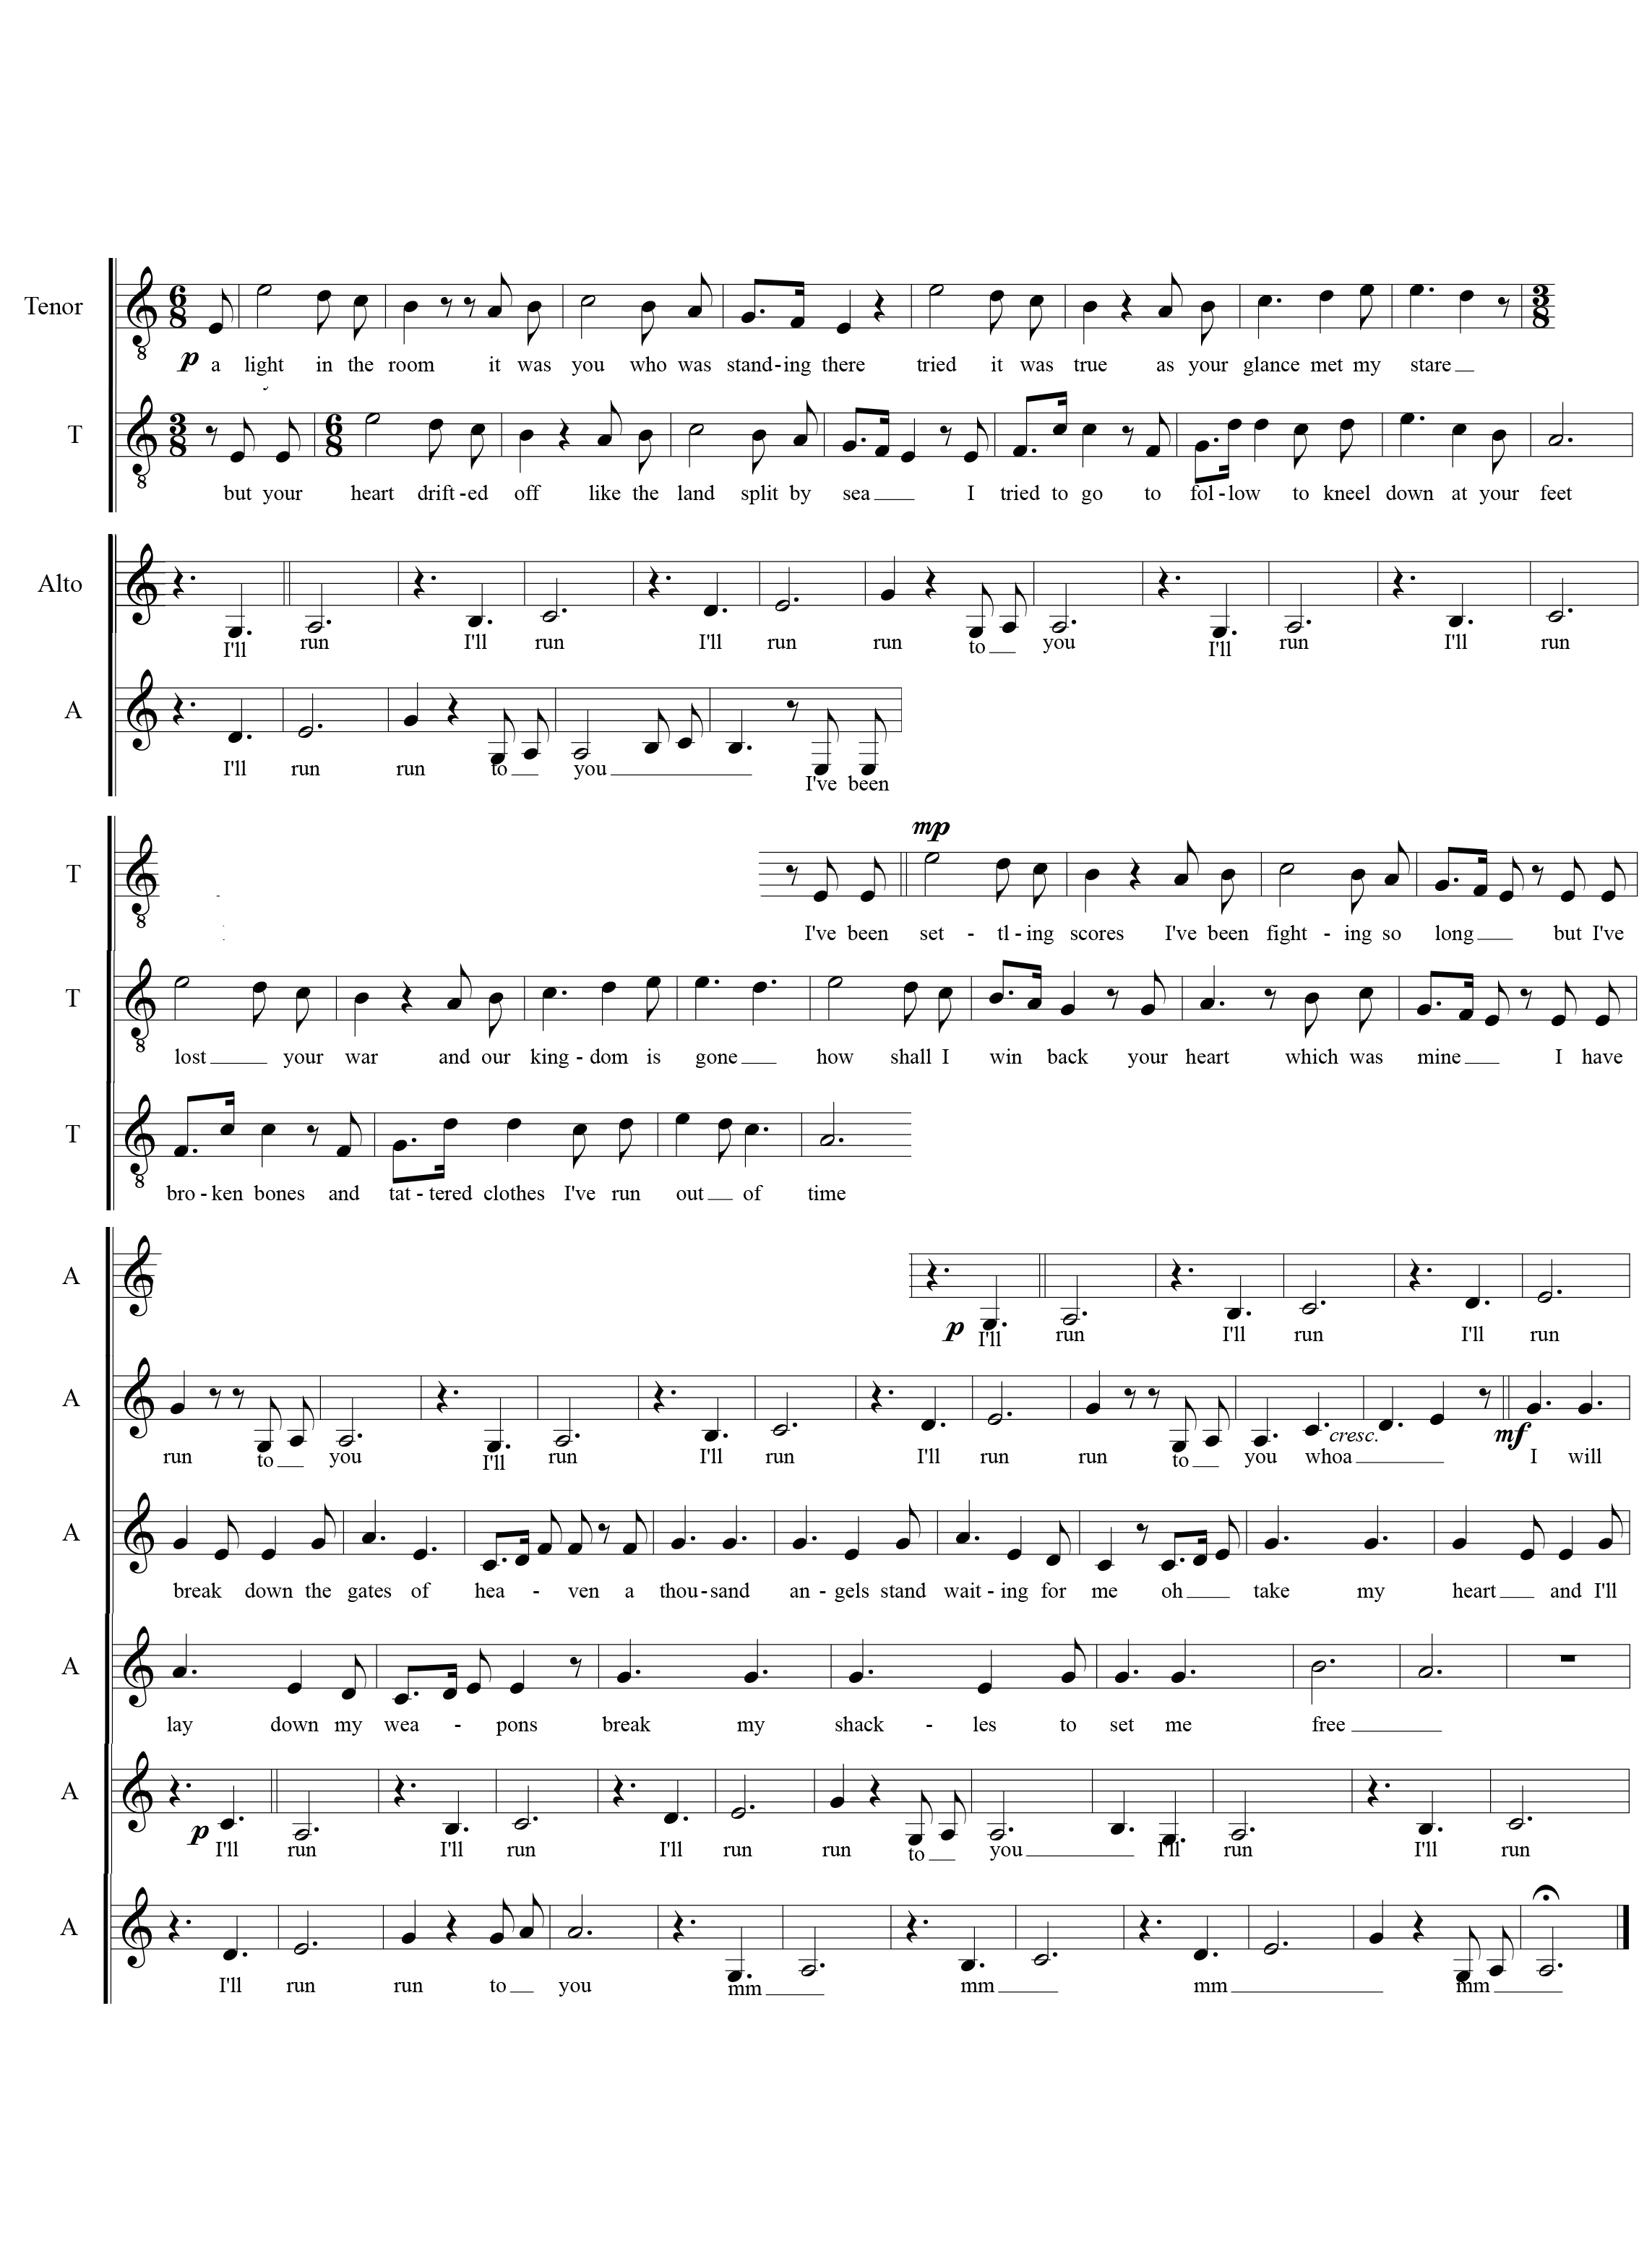
\includegraphics[width=\textwidth]{resources/arrangements/Run To You - Melody.png}
\label{appendix:Run To You}
 

\section{Fields Of Gold}

Das zweite Stück ist \textit{Fields Of Gold}, geschrieben von Gordon Sumner — bekannt unter dem Künstlernamen \textit{Sting} — und arrangiert von Greg Jasperse. Bei dem vorliegenden Arrangement handelt es sich um einen Satz für Sopran, Alt, Tenor und Bass. Das Stück besteht aus sechs Strophen, wobei sich zwischen der vierten und fünften Strophe eine Bridge befindet.

\begin{verbatim}
[Strophe 1]
You'll remember me when the west wind moves
Upon the fields of barley
You'll forget the sun in his jealous sky
As we walk in fields of gold

[Strophe 2]
So she took her love for to gaze awhile
Upon the fields of barley
In his arms she fell as her hair came down
Among the fields of gold

[Strophe 3]
Will you stay with me? Will you be my love?
Upon the fields of barley
We'll forget the sun in his jealous sky
As we lie in fields of gold

[Strophe 4]
See the west wind move like a lover so
Upon the fields of barley
Feel her body rise when you kiss her mouth
Among the fields of gold

[Bridge]
I never made promises lightly
And there have been some that I've broken
But I swear in the days still left
We'll walk in fields of gold
We'll walk in fields of gold

[Strophe 5]
Many years have passed since those summer days
Upon the fields of barley
See the children run as the sun goes down
Among the fields of gold

[Strophe 6]
You'll remember me when the west wind moves
Upon the fields of barley
You can tell the sun in his jealous sky
When we walked in fields of gold
When we walked in fields of gold
When we walked in fields of gold
\end{verbatim}